\documentclass[12pt]{article}
\usepackage[UTF8]{ctex}
\usepackage{geometry}
\usepackage{listings}
\usepackage{graphicx}
\usepackage{subfigure}
\usepackage{array}
\usepackage{caption}    
\usepackage{float}
\usepackage{subfloat}
\usepackage{hyperref}
\usepackage{bookmark}
\usepackage{amsmath}
\usepackage{url}
\usepackage{amsfonts,amssymb}

\geometry{left=15mm,right=15mm,top=20mm,bottom=20mm}
\title{期末项目报告\\ \large ——基于渐进式光子映射(SPPM)的图形渲染}

\author{PB21010410 高凡 \\PB21010362 汪兆辰}
\date{\today}
\newcommand{\upcite}[1]{\textsuperscript{\textsuperscript{\cite{#1}}}}

\begin{document}

\maketitle

\section{项目介绍}
\subsection{从基本全局光子映射(Basic Photon Mapping)讲起}
有效的实现全局光照(Global Illumination)的模拟是计算机图形学中的一个经典问题,在1998年Veach的博士论文中给出了无偏(unbiased)Monte-Carlo模拟的Path Tracing算法,但PT算法路径追踪在模拟散焦(caustics)时并不准确,同时
由于Monte-Carlo采样的误差阶是$\mathcal{O} (n^{-\frac{1}{2}})$,增加采样点对最终渲染结果的效果有限。

\begin{figure}[htbp]
    \centering
    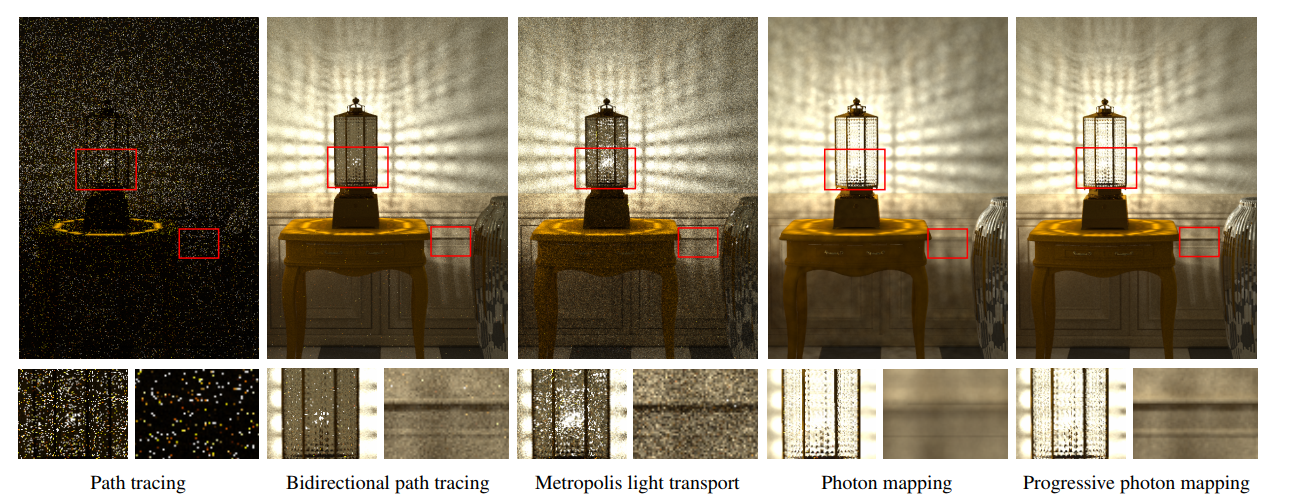
\includegraphics[scale=0.6]{pic1.png}
    \caption{几种光子映射算法的效果对比}
\end{figure}

对这种算法的一种改进是光子映射(Photon Mapping), 最朴素的光子映射分为两个阶段:第一个阶段需要构建一张光子贴图,用来存储从光源发射出的所有光子的通量信息;第二阶段从相机进行传统的路径追踪,在追踪到漫反射表面时统计附近的光子信息,并根据这些信息计算辐射率(radiance). 

\subsubsection{光子贴图}

构建光子贴图的基本思路是:让光源发出光子,并让光子在场景中反复弹射,直到被某个漫反射表面彻底吸收为止. 首先需要基于光源采样以确定光子的射线与初始功率,其中射线按照光源随机采样,而初始功率根据
\begin{equation}
    \Phi = \frac{L_e |\cos \theta|}{pdf_A (x)pdf_\omega (\omega)}
\end{equation}
来确定,其中$L_e$为光源自身的辐射率. 

在获得光子的初始状态后,需要对每一束光子在场景中反复迭代。当射线与表面相交时,按照表面的材质生成反射分布BSDF,并基于该BSDF记录下反射的方向与类型。如果反射类型为漫反射,就将光子的位置、路径与功率记录到光子贴图中,并随机按照反射比例判断是否终止迭代,如果未被吸收,则更新光子的功率,算法如下:

首先计算当前材质的反射率:
\begin{equation}
    R=\frac{f(x_{i-1}\rightarrow x_i \rightarrow x_{i+1})|\cos \theta|}{pdf_\omega (x_i \rightarrow x_{i+1})}
\end{equation}

然后得出光子的下一次功率:
\begin{equation}
    \Phi_{i+1}=\Phi_i \frac{R}{N_{BxDF}}
\end{equation}
其中$N_{BxDF}$为当前交点的反射分布下的反射模型的总数.

为了存储光子贴图,并加速光子映射,一种存储方式是按照光子图的位置构建平衡kd树,并用kNN算法进行优化,虽然建树的时间略微增加,但这种方式可以将后续查询的时间复杂度降到$\mathcal{O}(\sqrt{N}+K)$.

\subsubsection{基本全局光子映射}

由渲染方程:
\begin{equation}
    L_r(x,\omega)=\int_\Omega f(x,\omega',\omega)L_i(x,\omega')|\cos \theta'|d\omega'
\end{equation}
将辐射率
\begin{equation}
    L_i(x,\omega')=\frac{d^2 \Phi_i(x,\omega')}{dA|\cos \theta'|d\omega'}
\end{equation}
代入渲染方程得:
\begin{align}
    L_r(x,\omega)&=\int_\Omega f(x,\omega,\omega')\frac{d^2 \Phi_i(x,\omega')}{dA|\cos \theta'|d\omega'}|\cos \theta'|d\omega'\\
    &=\int _\Omega f(x,\omega,\omega')\frac{d^2\Phi_i(x,\omega')}{dA}
\end{align}
将其离散化得到:
\begin{equation}
    L_r(x,\omega)=\sum_{p=1}^{N}f(x,\omega_p,\omega)\frac{\Delta \Phi_p(x_p,\omega_p)}{\Delta A}
\end{equation}
其中$\Phi_p,\omega_p$分别为光子的功率与方向.

利用kd树和上述公式,取定合适的N就可以得到$L_r$, 样本N数量越多,估算的结果越接近真实值. 而由kd树的kNN算法可以得到样本所占的面积$\Delta A$,其中半径为
\begin{equation}
    r=\max(Dist(x,x_1),Dist(x,x_2),\ldots ,Dist(x,x_N))
\end{equation}

\subsubsection{全局光子映射的局限性}
作为最原始的光子映射方案,全局光子映射保留了相当明显的光子映射特征:由于样本的随机性与密度估计的插值效应,在样本较少的情况下,光子映射会出现明显的块状斑点(如图1-4).
另一方面,当场景中的大多数表面为光滑材质时,第一阶段中生成光子贴图需要多次迭代才能使得光子最终被吸收,而单纯为迭代次数设置上限会使得图像整体偏暗,需要更好的改进办法.

\begin{figure}[htbp]
    \centering
    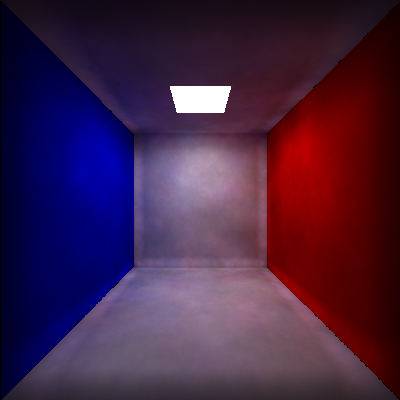
\includegraphics[scale=0.6]{pic2.png}
    \caption{全局光子映射渲染效果}
\end{figure}
其次,如图2所示,全局光子映射在场景的墙角处有明显的渗色情况,出现这种情况的原因是在密度估计过程中样本数量取的过大,使得部分与被估计光子不在同一平面的光子也参与了估计。在不占用大量内存与渲染时间的前提下很难有效果较好的优化,
所以需要对算法进一步改进。

\subsection{随机渐进式光子映射(SPPM)}
SPPM在PM的基础上调整了计算的模型,使得计算的结果可以近似完全收敛。首先要从PM过渡到渐进式光子映射(PPM),将PM中单次的光子映射改为多次光子映射并叠加,实现渐进式的收敛;之后再进一步将射线追踪阶段也拆为多次,并将PPM中基于场景的计算方式改为基于像素计算,以获得更低的开销与更快的收敛速度。

\subsubsection{从PM到PPM}
在\cite{7}中,Jensen提出了一种改进措施,将PM的光子映射拆成多次,形成多张光子图并分批执行密度估计,对所有结果取平均值,但这最多将估计范围收敛到对应的kNN范围r内,而如果一开始将r取的很小,会使得估计范围内光子密度很低,降低估计效率,所以
实现对估计半径r的控制成为了重点的问题。

改进方案的前几步与Jensen 2004相同:假设第一次密度估计需要$N_1(x)$个光子,在第一轮密度估计后,利用kNN算法可以得到估计范围的半径$R_1(x)$,并得到第一次估计的密度$d_1(x)=\frac{N_1(x)}{\pi R_1(x)^2}$.之后维持半径$R_1(x)$不变,重新生成一张光子图,并围绕新的光子图基于同样的半径$R_1(x)$做一次密度估计,假设新的光子数目为$M_1(x)$,
则新的密度估计为
\begin{equation}
    d_2(x)=\frac{N_1(x)+M_1(x)}{\pi R_1(x)^2}
\end{equation}


在进行下一步密度估计之前,先对估计半径进行收缩,假设在收缩过程中密度是不变的,可以计算出半径缩减后下一轮光子个数$N_2(x)$与密度$d_2(x)$的关系:
\begin{equation}
    d_2(x)=\frac{N_2(x)}{\pi R_2(x)^2}=\frac{N_2(x)}{\pi (R_1(x)-\Delta R_1(x))^2}
\end{equation}
其中$\Delta R_1(x)$为第一次迭代过渡到第二次过程中半径的缩减量.而下一轮光子数量$N_2(x)$取决于上一轮光子$N_1(x)$与新增光子$M_1(x)$,这里$N_1(x)$无法更改,但可以控制新增部分的比例,即
\begin{equation}
    N_2(x)=N_1(x)+\alpha M_1(x)
\end{equation}
其中缩减系数$\alpha$实际上控制了半径$R_2(x)$的衰减速度.结合(10)-(12)三式,可得:
\begin{equation}
    R_2(x)=R_1(x) \sqrt{\frac{N_1(x)+\alpha M_1(x)}{N_1(x)+M_1(x)}}
\end{equation}
重复此过程,可以使得估算半径不断收敛。

记x处出射到相机方向$\omega$的总通量为:
\begin{equation}
    \tau(x,\omega):=\sum_{p=1}^{N} f(x,\omega_p,\omega)\Delta \Phi_p(x,\omega_p) 
\end{equation}
假设已经迭代了i轮,累积了$N_i(x)$个光子,那么这些光子的总通量理论上可以计算为:
\begin{equation}
    \tau_i(x,\omega)=\sum_{p=1}^{N_i(x)} f(x,\omega_p,\omega)\Delta \Phi_p(x,\omega_p)
\end{equation}
然后下一步,缩减前新增$M_i(x)$个光子,尽管由于半径缩减最终只保留其中的一部分,但依然需要计算全部新增光子的总通量,记为: 
\begin{equation}
    \phi_i(x,\omega)=\sum_{p=1}^{M_i(x)} f(x,\omega_p,\omega)\Delta \Phi_p(x,\omega_p)
\end{equation}
由公式(13)可以计算出收敛后半径:
\begin{equation}
    R_{i+1}(x)=R_i(x)\sqrt{\frac{N_i(x)+\alpha M_i(x)}{N_i(x)+M_i(x)}}
\end{equation}
并估计出缩减后保留的总通量:
\begin{equation}
    \tau_{i+1}(x,\omega)=(\tau_i(x,\omega)+\phi_i(x,\omega))\frac{N_i(x)+\alpha M_i(x)}{N_i(x)+M_i(x)}
\end{equation}
结合式(8)可以计算出第i+1轮的辐射率:
\begin{align}
    L_r(x,\omega)&=\frac{1}{\Delta A}\sum_{p=1}^{N_{i+1}(x)}f(x,\omega_p,\omega)\Delta \Phi_p(x,\omega_p)\\
    &=\frac{1}{\pi R_{i+1}(x)^2}\frac{\tau_{i+1}(x,\omega)}{N_e(i+1)}
\end{align}
随着迭代次数不断增大,总通量$\tau_{i+1}(x,\omega)$增大,密度估计半径$R_{i+1}(x)$缩小,全局光子总数$N_e(i+1)$越来越多,能够完全收敛。

但由于PPM需要为每个像素点分配很多射线与漫反射面相交形成的命中点才能有效去噪,仍然需要较大的内存开销。
\subsubsection{从PPM到SPPM}
SPPM在PPM的基础上改进了对命中点的生成,在每个渲染阶段,先进行一次射线追踪,再对每次射线追踪生成一小批命中点,并围绕这些命中点在一个像素范围内抖动更新,从而当样本量足够大时,估算的即为像素内的全部区域。
而SPPM的计算公式与PPM的式(20)只需将命中点x改为像素区域S:
\begin{equation}
    L_r(S,\omega)=\frac{1}{\pi R_{i+1}(S)^2}\frac{\tau_{i+1}(S,\omega)}{N_e(i+1)}
\end{equation}

\section{代码介绍}

项目代码由以下部分组成:
\begin{itemize}
    \item aabb.hpp
    \item bvh.hpp
    \item camera.hpp
    \item photon.hpp
    \item photon\_map.hpp
    \item ray.hpp
    \item renderable.hpp
    \item SppmManager.hpp
    \item SPPM.cpp
    \item 外部Eigen与stb库
\end{itemize}

\subsection{aabb.hpp}
该头文件定义了Axis Aligned Bounding Box对象,其中成员包括:
\begin{itemize}
    \item v6f limits:六个面的限定参数
    \item bool is\_ray\_inter(Ray\& ray):测试是否与射线相交
    \item AABB union\_with\_other(AABB\& another):融合两个AABB
    \item v3f get\_center():获取AABB的中心
\end{itemize}

\subsection{bvh.hpp}
该头文件定义了BVH树对象以及相关的类型,包括:
\begin{itemize}
    \item struct BVHNd:BVH树节点结构体
    \begin{itemize}
        \item BVHNd* lc, * rc; 左右孩子
        \item AABB aabb; 节点对应的AABB
        \item Renderable *rd\_obj; 包围盒中的物体。该指针仅有在节点为叶子时才非空
    \end{itemize}
    \item struct IntersectInfo: 相交信息记录
    \begin{itemize}
        \item Renderable* obj; 相交的物体
        \item v3f pos; 相交位置
        \item float distance; 射线发出点到相交点的位置
        \item bool do\_intersect; 是否真的相交的标志位。如果为false说明该射线事实上与场景并没有交点
    \end{itemize}
    \item class BVH
    \begin{itemize}
        \item BVHNd* root; 根节点
        \item std::vector<Renderable*> obj\_ptr\_list; 可渲染物体指针的列表。该列表是参数的复制,因为需要对列表进行排序。
        \item std::vector<BVHNd*> tree\_nodes; 所有的树节点
        \item IntersectInfo get\_first\_intersection(Ray\& ray, Renderable* obj) 获取射线的交点,同时排除当前物体obj
    \end{itemize}
\end{itemize}

\subsection{camera.hpp}
该头文件定义了相机对象
\begin{itemize}
    \item class Cam
    \begin{itemize}
        \item v3f top, lookat, pos; 相机几何参数
        \item int w, h; 图像参数
        \item float focus, fov; 焦点与fovY
        \item float ccd\_w, ccd\_h; 相机ccd参数
        \item v3f local\_x\_ax; 相机坐标系未显式给出的轴
        \item Ray sample\_ray\_xy(int x, int y, float fltx, float flty) 计算某一个像素点采样射线
    \end{itemize}
\end{itemize}

\subsection{photon.hpp}
该头文件定义了光子
\begin{itemize}
    \item class Photon
    \begin{itemize}
        \item v3f power\_rgb; 光子携带的能量
        \item Ray ray; 光子对应的传播射线
        \item v3f end\_at; 光子击中位置
        \item bool bounce; 是否击中某个目标
    \end{itemize}
\end{itemize}

\subsection{photon\_kdt.hpp}

该头文件定义了光子对象的kdtree
\begin{itemize}
    \item struct KDTNd kdt节点
    \begin{itemize}
        \item Photon *ph 对应的光子
        \item int axis; 分割轴
        \item KDTNd* lc, * rc; 左右孩子
    \end{itemize}
    \item class KDT
    \begin{itemize}
        \item KDTNd *root; 根节点
        \item std::vector<KDTNd*> ptrs; 节点指针
        \item KDTNd* recursive\_construction(int st, int ed, std::vector<Photon>\& photons, int axis) 构建kdt
        \item void recursive\_kdt\_search(pq\_kdt\& pq, int N, KDTNd* nd, v3f\& pos) 搜索给定数目的节点
        \item std::vector<Photon*> N\_near(int N, v3f pos) 搜索定额
        \item std::vector<Photon*> N\_near\_with\_R(int N, v3f pos, float R) 搜索定额以及半径以内
    \end{itemize}
\end{itemize}

\subsection{photon\_map.hpp}
该头文件定义了光子图的生成
\begin{itemize}
    \item class PhotonMap
    \begin{itemize}
        \item std::vector<Photon> photon\_record; 光子记录
        \item void get\_map\_mt(int n\_th, int n, Scene\& sc, int single\_max\_iter = 32, float rr\_prob = 0.8) 多线程生成光子,计算传播,记录光子
    \end{itemize}
\end{itemize}


\subsection{ray.hpp}
该头文件定义了射线
\begin{itemize}
    \item class Ray
    \begin{itemize}
        \item v3f pos; 起点
        \item v3f dir; 方向
        \item v3f get\_t(float t) 获取在距离t处的位置
    \end{itemize}
\end{itemize}

\subsection{renderable.hpp}
该头文件定义了所有可渲染物体的基类Renderable以及对应的受支持模型类型——三角网格\&球体的派生类Triangle\&Ball
\begin{itemize}
    \item class Renderable
    \begin{itemize}
        \item int n\_materials; 材质的数目
        \item bool has\_spec;
        \item bool has\_lamb;
        \item bool has\_tran; 是否具有支持的三种材质:镜面反射、理想漫反射、透射
        \item bool is\_light; 是否是光源
        \item float spec\_ratio;
        \item float lamb\_ratio;
        \item float tran\_ratio; 采样BSDF时的概率
        \item v3f color; 颜色参数
        \item float emit\_power; 发光强度
        \item float n\_t; 折射率
        \item virtual InteractType sample\_reflect\_type() 采样BSDF
        \item virtual Ray get\_next\_ray(InteractType type,  Ray\& in, v3f pos) 根据反射类型以及入射信息计算出射射线
        \item virtual v3f get\_bsdf(InteractType type, v3f in\_dir, v3f out\_dir, v3f pos) 获取对应BSDF
        \item virtual std::pair<float, v3f> try\_intersect\_ray(Ray\& in) 获取交点以及距离
        \item virtual Photon emit\_a\_photon() 发射光子,仅当是光源时才使用
        \item virtual v3f get\_norm(v3f pos) 获取曲面某点的法向
        \item virtual v3f sample\_a\_pos() 随机采样曲面上一点
        \item virtual float A() 面积
        \item std::vector<std::pair<InteractType, float>> available\_mat; 可使用的材质
    \end{itemize}
    \item class Triangle: public Renderable
    \begin{itemize}
        \item v3f v0, v1, v2; 顶点
        \item v3f norm; 预先计算的法向
    \end{itemize}
    \item class Ball :public Renderable
    \begin{itemize}
        \item v3f center; 球心
        \item float radius; 半径
    \end{itemize}
\end{itemize}

\subsection{scene.hpp}
该头文件定义了场景对象
\begin{itemize}
    \item class Scene
    \begin{itemize}
        \item std::vector<Renderable* > objs; 可渲染物体
        \item std::vector<Renderable* > light\_src; 光源
        \item BVH *bvh; BVH树
        \item void append\_obj(Renderable* obj) 添加物体
        \item void construct\_bvh() 建立BVH
        \item static std::vector<Renderable*> parse\_triangle\_file(std::string filename) 解析三角网格文件    
    \end{itemize}
\end{itemize}

\subsection{SppmManager.hpp}
该头文件定义了所有与随机渐进光子映射有关的过程
\begin{itemize}
    \item constexpr float dec\_fac = 0.75f; 半径衰减系数
    \item struct Q 采样路径的一些记录
    \begin{itemize}
        \item v3f pos, dir;采样的几何信息
        \item Renderable* obj; 击中物体
        \item v3f beta; 吞吐量
        \item bool islt; 是否击中光源,如果是,则光源的radiance额外计算
    \end{itemize}
    \item struct SppmPix SPPM像素 
    \begin{itemize}
        \item v3f direct\_radiance; 直接光照radiance
        \item int direct\_radiance\_cnt; 光照计数
        \item bool is\_first\_estimate; 是否第一次估计
        \item float global\_shared\_radius 估计半径
        \item v3f global\_cumulate\_pow; 积累的通量
        \item int global\_N; 累计光子数目
        \item int needed\_N; 下次搜索时的搜索上界,目的是优化搜索速度
        \item std::vector<Q> sample\_position\_dir\_obj\_beta;  预采样信息
    \end{itemize}   
    \item class SppmManager SPPM的主要处理逻辑
    \begin{itemize}
        \item Cam camera; 相机
        \item std::vector<SppmPix> sppm\_pix\_list; 像素
        \item int single\_sp; 单点采样上限
        \item inline int get\_pix\_id(int x, int y) { return y * camera.w + x; } 获取像素点位置
        \item void initialize\_samples\_mt(Scene \& sc, int th = 8, int single\_samples = 32, int max\_ray\_reflect = 16) 多线程预采样
        \item void single\_run(Scene\& sc, int th = 8,
              const int global\_scale = 50000,\\
              const int global\_map\_iter = 32,
              const int global\_search\_N = 100,\\
              const float global\_search\_R = 0.05,
              const int all\_sp = 32)
              多线程单次迭代
        \item v3b get\_value(float scale , int x, int y) 获取最后的像素值
      
    \end{itemize}
\end{itemize}

\subsection{SPPM.cpp程序入口}
\begin{itemize}
    \item [1.] 加载渲染物体到场景
    \item [2.] 构建bvh
    \item [3.] 定义相机
    \item [4.] 创建SppmManager
    \item [5.] 预采样
    \item [6.] 根据迭代次数进行计算
    \item [7.] 根据给定比例计算输出图像并储存
\end{itemize}

\section{效果展示}
渲染的图像效果如下:
\begin{figure}[htbp]
    \centering
    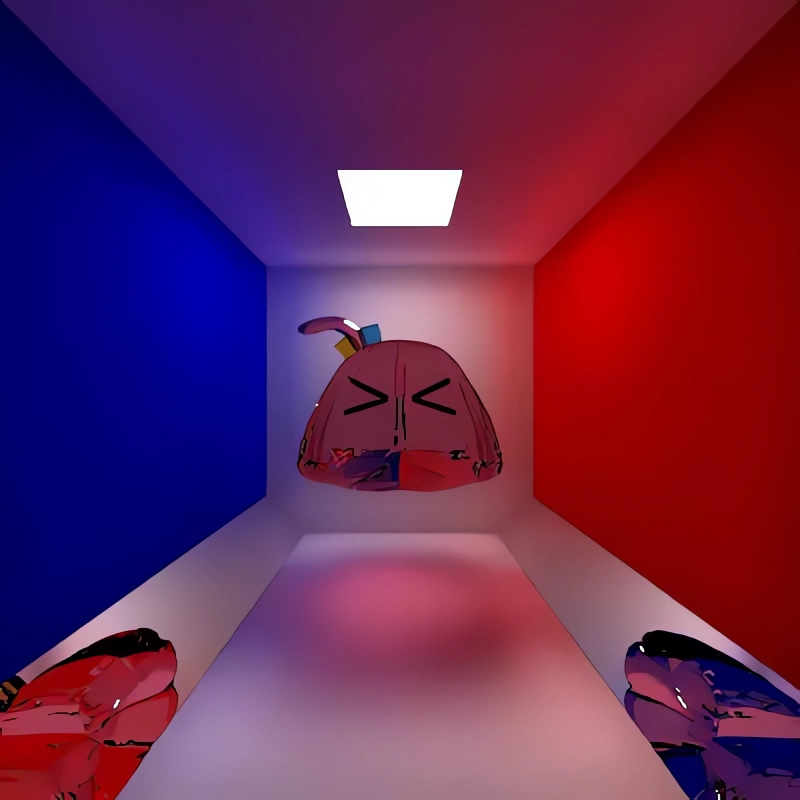
\includegraphics[scale=0.6]{pic3.png}
    \caption{bocchi pudding}
\end{figure}

\begin{figure}[htbp]
    \centering
    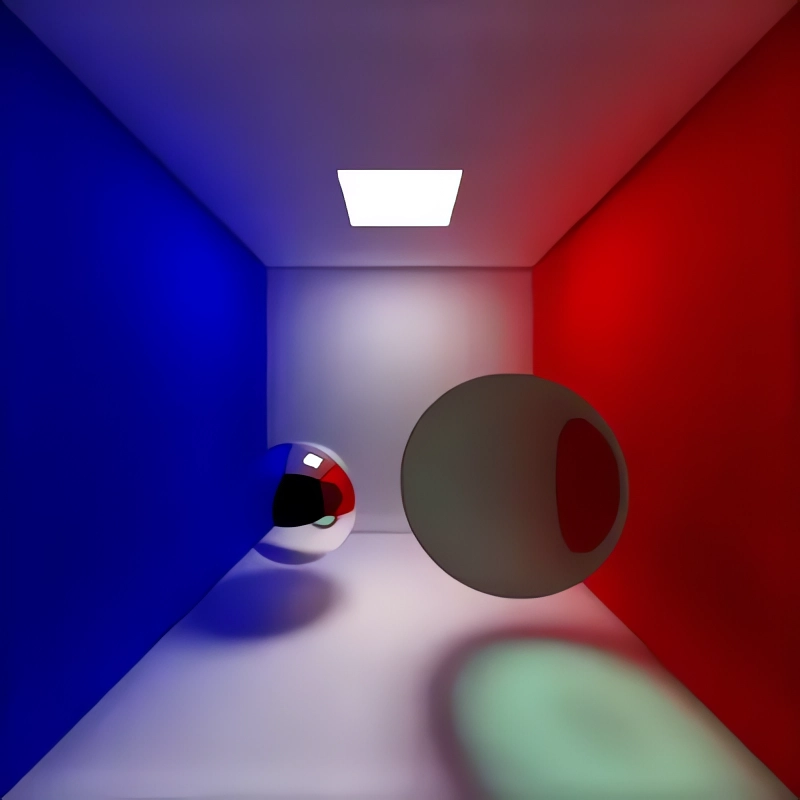
\includegraphics[scale=0.6]{pic4.png}
    \caption{greenball}
\end{figure}


\newpage

\section*{致谢}
{\large
\begin{itemize}
    \item 感谢陈老师与两位助教一学期的悉心教导
    \item 感谢知乎答主@我好饱啊的光子映射总结. Talk is not cheap. Talk can be powerful.
    \item 感谢临近期末中区自习室晚上不断电可以跑一晚上的图
    \item 感谢《孤独摇滚》及其全体制作人员,有你们业界完不了
    \item 感谢三井律郎在「忘れてやらない」编曲的巨大升级,让我练不下去来写报告
    \item 感谢肥西路,南边第一家热干面和凉皮做的真不错
    \item 首先我是一个无神论者,然后感谢所有保佑代码不出bug的神灵,我愿称之为代码仙人
\end{itemize}
}

\begin{thebibliography}{3}
    \bibitem{1} \url{https://zhuanlan.zhihu.com/p/208356944}
    \bibitem{2} \url{https://zhuanlan.zhihu.com/p/259565623}
    \bibitem{3} \url{https://graphics.stanford.edu/courses/cs348b-00}
    \bibitem{4} M.Pharr, W.Jakob, and G.Humphreys. Physically Based Rendering: From Theory To Implementation. 2018.
    \bibitem{5} T.Hachisuka, S.Ogaki, and H.W.Jensen. Progressive Photon Mapping. ACM SIGGRAPH Asia 2008 Papers, 2008.
    \bibitem{6} T.Hachisuka, H.W.Jensen. Stochastic progressive photon mapping. ACM Transactions on Graphics, 2009.
    \bibitem{7} H.W.Jensen. ACM SIGGRAPH 2004 Course Notes. A practical guide to global illumination using ray tracing and photon mapping, 2004.
    \bibitem{8} E.Veach. Stanford University. Robust monte carlo methods for light transport simulation, 1998.
\end{thebibliography}

\end{document}